\documentclass[11pt,border=6pt]{standalone}
\usepackage{fontspec}
\usepackage{tikz}
\begin{document}
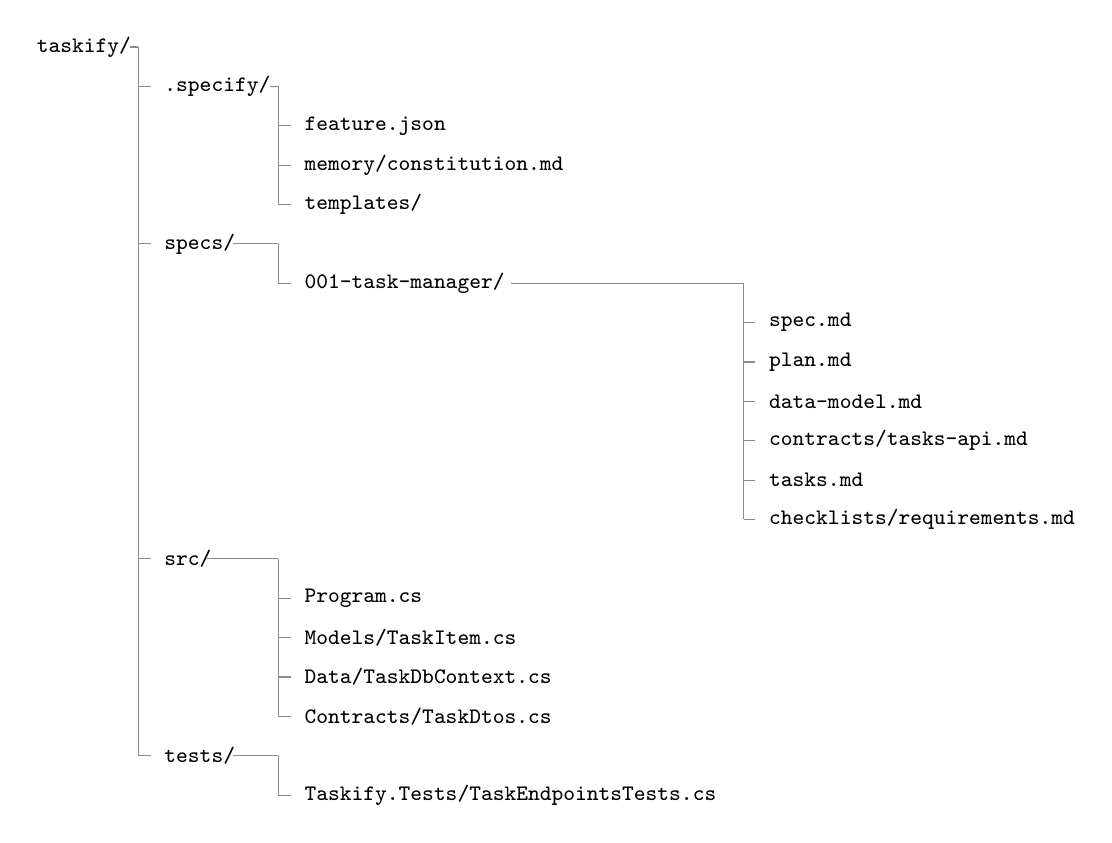
\begin{tikzpicture}

% nodi: nome in monospazio, annotazione in grigio
\node[anchor=west, font=\ttfamily\footnotesize] (n0) at (0.00,0.00) {taskify/};
\node[anchor=west, font=\ttfamily\footnotesize] (n1) at (1.62,-0.50) {.specify/};
\node[anchor=west, font=\ttfamily\footnotesize] (n2) at (3.40,-1.00) {feature.json};
\node[anchor=west, font=\ttfamily\footnotesize] (n3) at (3.40,-1.50) {memory/constitution.md};
\node[anchor=west, font=\ttfamily\footnotesize] (n4) at (3.40,-2.00) {templates/};
\node[anchor=west, font=\ttfamily\footnotesize] (n5) at (1.62,-2.50) {specs/};
\node[anchor=west, font=\ttfamily\footnotesize] (n6) at (3.40,-3.00) {001-task-manager/};
\node[anchor=west, font=\ttfamily\footnotesize] (n7) at (9.30,-3.50) {spec.md};
\node[anchor=west, font=\ttfamily\footnotesize] (n8) at (9.30,-4.00) {plan.md};
\node[anchor=west, font=\ttfamily\footnotesize] (n9) at (9.30,-4.50) {data-model.md};
\node[anchor=west, font=\ttfamily\footnotesize] (n10) at (9.30,-5.00) {contracts/tasks-api.md};
\node[anchor=west, font=\ttfamily\footnotesize] (n11) at (9.30,-5.50) {tasks.md};
\node[anchor=west, font=\ttfamily\footnotesize] (n12) at (9.30,-6.00) {checklists/requirements.md};
\node[anchor=west, font=\ttfamily\footnotesize] (n13) at (1.62,-6.50) {src/};
\node[anchor=west, font=\ttfamily\footnotesize] (n14) at (3.40,-7.00) {Program.cs};
\node[anchor=west, font=\ttfamily\footnotesize] (n15) at (3.40,-7.50) {Models/TaskItem.cs};
\node[anchor=west, font=\ttfamily\footnotesize] (n16) at (3.40,-8.00) {Data/TaskDbContext.cs};
\node[anchor=west, font=\ttfamily\footnotesize] (n17) at (3.40,-8.50) {Contracts/TaskDtos.cs};
\node[anchor=west, font=\ttfamily\footnotesize] (n18) at (1.62,-9.00) {tests/};
\node[anchor=west, font=\ttfamily\footnotesize] (n19) at (3.40,-9.50) {Taskify.Tests/TaskEndpointsTests.cs};

% connettori ad albero
\draw[black!45] (1.31,0.00) -- (1.41,0.00);
\draw[black!45] (1.41,0.00) -- (1.41,-9.00);
\draw[black!45] (1.41,-0.50) -- (1.57,-0.50);
\draw[black!45] (1.41,-2.50) -- (1.57,-2.50);
\draw[black!45] (1.41,-6.50) -- (1.57,-6.50);
\draw[black!45] (1.41,-9.00) -- (1.57,-9.00);
\draw[black!45] (3.09,-0.50) -- (3.19,-0.50);
\draw[black!45] (3.19,-0.50) -- (3.19,-2.00);
\draw[black!45] (3.19,-1.00) -- (3.35,-1.00);
\draw[black!45] (3.19,-1.50) -- (3.35,-1.50);
\draw[black!45] (3.19,-2.00) -- (3.35,-2.00);
\draw[black!45] (2.61,-2.50) -- (3.19,-2.50);
\draw[black!45] (3.19,-2.50) -- (3.19,-3.00);
\draw[black!45] (3.19,-3.00) -- (3.35,-3.00);
\draw[black!45] (6.14,-3.00) -- (9.10,-3.00);
\draw[black!45] (9.10,-3.00) -- (9.10,-6.00);
\draw[black!45] (9.10,-3.50) -- (9.25,-3.50);
\draw[black!45] (9.10,-4.00) -- (9.25,-4.00);
\draw[black!45] (9.10,-4.50) -- (9.25,-4.50);
\draw[black!45] (9.10,-5.00) -- (9.25,-5.00);
\draw[black!45] (9.10,-5.50) -- (9.25,-5.50);
\draw[black!45] (9.10,-6.00) -- (9.25,-6.00);
\draw[black!45] (2.29,-6.50) -- (3.19,-6.50);
\draw[black!45] (3.19,-6.50) -- (3.19,-8.50);
\draw[black!45] (3.19,-7.00) -- (3.35,-7.00);
\draw[black!45] (3.19,-7.50) -- (3.35,-7.50);
\draw[black!45] (3.19,-8.00) -- (3.35,-8.00);
\draw[black!45] (3.19,-8.50) -- (3.35,-8.50);
\draw[black!45] (2.61,-9.00) -- (3.19,-9.00);
\draw[black!45] (3.19,-9.00) -- (3.19,-9.50);
\draw[black!45] (3.19,-9.50) -- (3.35,-9.50);
\end{tikzpicture}
\end{document}
